\chapter{Analysis}

\section{Introduction}

\subsection{Client Identification}
My client is Terry Jacobs. He is the group leader of the Fordham scout group, of approximately 55 children, and is required to oversee the running of the group and its daughter groups. He is also in charge of billing, as the parents must pay  \pounds 30 a school term for their child to be enrolled. However, if a member that wishes to join has a sibling who is also a member, a discount is given for the the new member. This must be notified by the parent however, and is not automatically displayed, and should also affect half-siblings or siblings who do not share the same surname.

Terry would like a new system to clearly display which members need a sibling discount and for the system to also format invoices for easy printing, or for the system to instead email the invoice, however this would require all the parents having an email. If the system could automate all this it would save Terry time and also help prevent any mistakes that may be made.

\subsection{Define the current system}
The current system is a manual operation. Records of clients are kept on paper in Terry's office and in a excel spread on his home laptop. Records include:
\begin{itemize}
   \item first name of member
   \item last name of member
   \item first name of parent
   \item last name of parent
	\item address of member
	\item address of parent
	\item phone number of parent
	\item email of parent
	\item age of member
	\item whether the member gets a sibling discount
	\item amount to be paid
	\item whether the invoice has been paid for that term
	\item when the last invoice was paid
	\item any outstaiding payments
	\item additional information
\end{itemize}

Members who have left are also recorded and kept for twelve months, and the data's accuracy should be checked every twelve months to make sure the member hasn't moved or their data has been changed and the organisation has not been notified.

If a new member wishes to join, Terry can be emailed by the parent of the member who can then provide details so Terry can record the information in the database.

Data is first manually recorded onto the excel spreadsheet. The excel spreadsheat
Any data that is needed for the invoice is copied to a template word document from the excel spreadsheet, ususally this data is the name of the parents and member, the address, the. The word document is then printed to be ready

Every year the parent is billed \pounds 30 for their child to be enrolled. This is done by an invoice. Usually this is done by post, an invoice is sent to the address in an unsealed envelope for a cheque or cash to be returned to the return address. However, this can lead to mistakes and is time consuming as well as costing money to print 55 invoices.

\subsection{Describe the problems}
Keeping the records in a non-secure place is not ideal, especially as some of the child's secure information such as the name and address is kept on record.

Obviously, this manual approach to sending the invoices has difficulties as with over 100 invoices to print, plus 100 envelopes to buy and prepare this can be time consuming and expensive. Errors can and have been made in the past.


\subsection{Section appendix}

\section{Investigation}

\subsection{The current system}

\subsubsection{Data sources and destinations}

\begin{table}[h]
\begin{tabular}{|p{1.5cm}|p{3.5cm}|p{5cm}|p{2cm}|l}
\hline
\textbf{Source} & \textbf{Data}  & \textbf{Example Data}  & \textbf{Destination}     \\ \hline
Client           &  \begin{itemize}
	\item Member first name
	\item Member last name
	\item Parents first name
	\item Parent last name
	\item Member address
	\item Parent address
	\item Parent phone number
	\item Parent email
	\item Member age
	\item Sibling discount
	\item Last invoice paid
\end{itemize} & 
\begin{itemize}
	\item John
	\item Smith
	\item Sarah
	\item Smith
	\item 123 Example Road
	\item 01234 123456
	\item sarahsmith@longroad.ac.uk
	\item 14
	\item True
	\item 1st January 2014
\end{itemize} & 
Database \\ \hline
Database &
\begin{itemize}
	\item Amount to be paid
	\item Parent address
	\item Return address
\end{itemize} & 
\begin{itemize}
	\item \pounds 30
	\item 123 Example Road
	\item 123 Payment Road
\end{itemize} & 
Invoice template \\ \hline
Invoice Template & 
\begin{itemize}
	\item Amount to be paid
	\item Parent address
	\item Return address
\end{itemize} & 
\begin{itemize}
	\item \pounds 30
	\item 123 Example Road
	\item 123 Payment Road
\end{itemize} & 
Printed Invoice \\
\hline
\end{tabular}
\end{table}

\subsubsection{Algorithms}
There are three algorithms in the current system:

Is the member old enough to join?
IF (Age of member = Old enough to join) THEN
	Allow to join = True
ELSE
	Allow to join = False

Does the member need a sibling discount?
IF (Client does have a sibling member) THEN
	Discount = True
ELSE
	Discount = False
END IF


\begin{algorithm}[H]
    \caption{Deciding which team won}
\begin{algorithmic}[1]
\If{$team\_one\_score > team\_two\_score$}
\SET{$winner$}{$team\_one$}
\ElsIf{$team\_one\_score < team\_two\_score$}
\SET{$winner$}{$team\_two$}
\Else
\SET{$winner$}{$"Draw"$}
\EndIf
\end{algorithmic}
\end{algorithm}

Has the parent payed?
WHILE (Invoice Payed = False) DO
	Contact Parent for payment
	IF (Parent does not want to pay) THEN
		Member is rejected
	ELSE
		IF (Parent did not get invoice) THEN
			Reprint invoice and send to parent
		ELSE
			Wait for invoice
		END IF
	END IF
END WHILE

\subsubsection{Data flow diagram}

Key:


Adding a new member:
\begin{figure}[H]

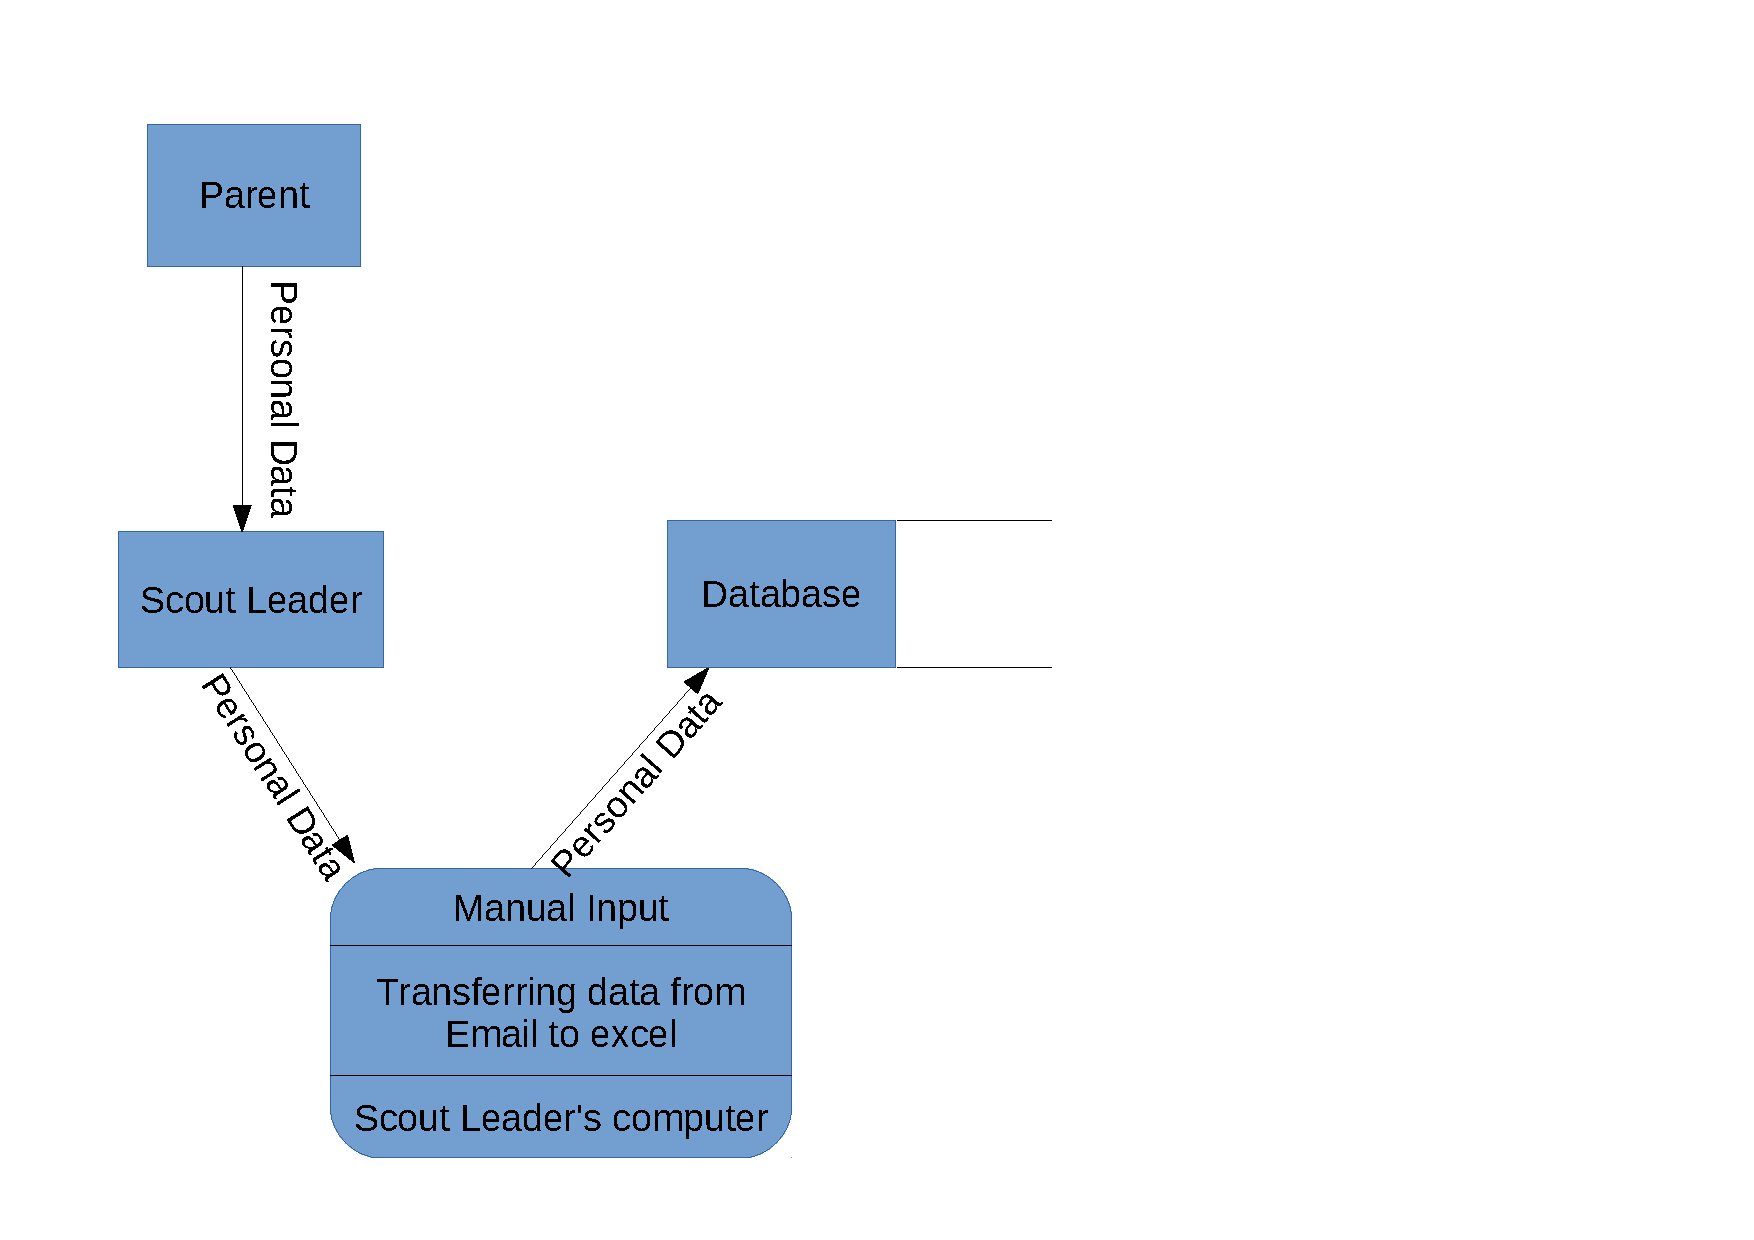
\includegraphics[width=\textwidth]{./Analysis/Images/Data_Flow_Adding_New_Member.pdf}
    \caption{Adding a new member} \label{fig:add_new_member}
\end{figure}

Printing an invoice:
\begin{figure}[H]
    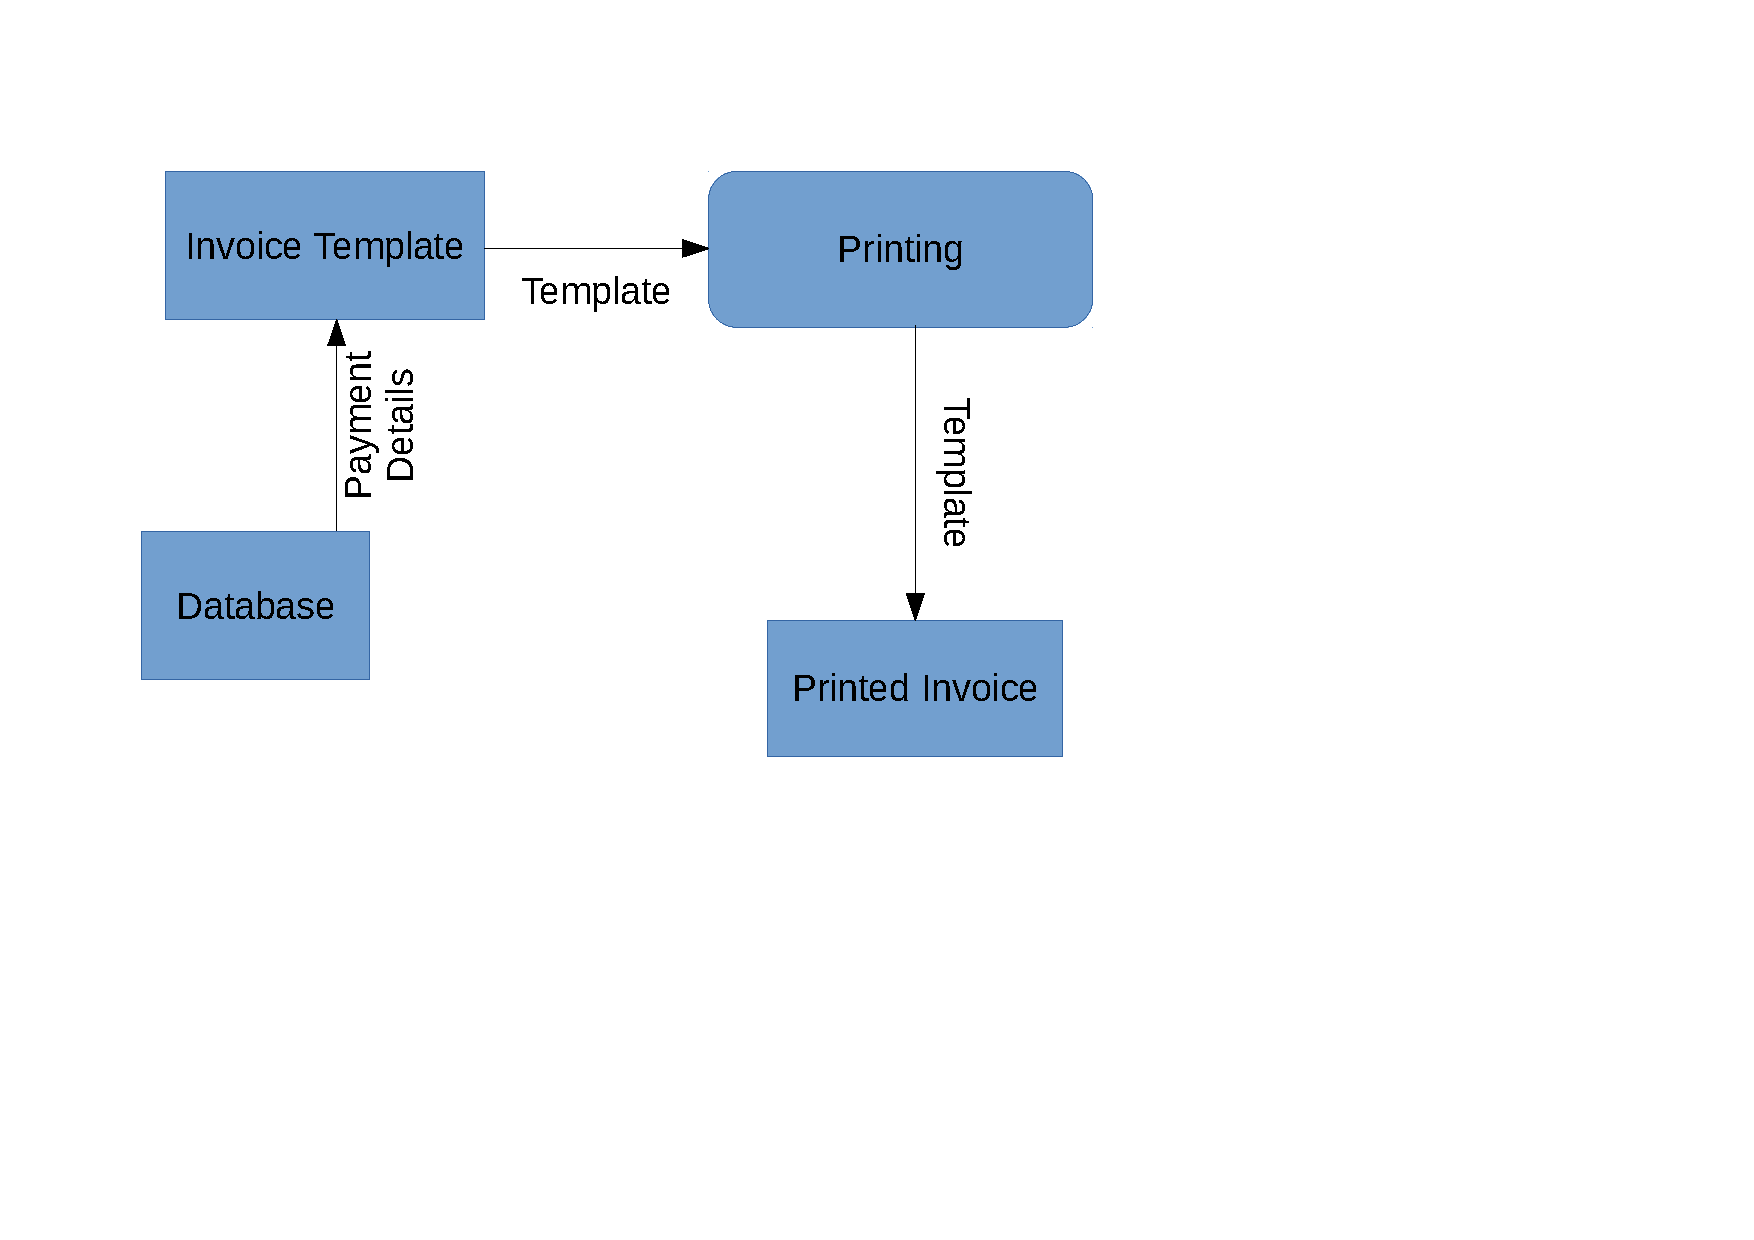
\includegraphics[width=\textwidth]{./Analysis/Images/Data_Flow_Printing_Invoice.pdf}
    \caption{Printing an invoice from the database} \label{fig:printt_invoice}
\end{figure}

\subsubsection{Input Forms, Output Forms, Report Formats}
Input Forms:
The System has no formal input forms, however parents must send Terry their data in an email.

Output Forms:
The system has one output form, the invoice.
{Invoice Scan}


\subsection{The proposed system}

\subsubsection{Data sources and destinations}

\begin{table}[h]
\begin{tabular}{llll}
Source          & Data                      & Data Type & Destination     \\
Member's Parent & Member first name         & String    & Member Database \\
Member's Parent & Member last name          & String    & Member Database \\
Member's Parent & Parents first name        & String    & Member Database \\
Member's Parent & Parent last name          & String    & Member Database \\
Member's Parent & Member address            & String    & Member Database \\
Member's Parent & Parent address            & String    & Member Database \\
Member's Parent & Parent phone number       & Integer   & Member Database \\
Member's Parent & Parent email              & String    & Member Database \\
Member's Parent & Member age                & Integer   & Member Database \\
Member's Parent & Number of sibling members & Integer   & Member Database \\
Member's Parent & Last invoice paid         & Integer   & Member Database \\
Database        & Amount to be paid         & Integer   & Invoice Template \\
Database        & Parent address            & String    & Invoice Template \\
Database        & Return address            & String    & Invoice Template \\
Database        & Parent first name         & String    & Invoice Template \\
Database        & Member first name         & String    & Invoice Template \\
Database        & Parent last name          & String    & Invoice Template \\
Database        & Member last name          & String    & Invoice Template \\
Database        & Invoice ID                & Integer   & Invoice Template \\
Database        &                           &           & Invoice Template \\
Database        &                           &           & Invoice Template \\

\end{tabular}
\end{table}

\subsubsection{Data flow diagram}

\subsubsection{Data dictionary}

\subsubsection{Volumetrics}

\section{Objectives}

\subsection{General Objectives}

\subsection{Specific Objectives}

\subsection{Core Objectives}

\subsection{Other Objectives}

\section{ER Diagrams and Descriptions}

\subsection{ER Diagram}

\subsection{Entity Descriptions}

\section{Object Analysis}

\subsection{Object Listing}

\subsection{Relationship diagrams}

\subsection{Class definitions}

\section{Other Abstractions and Graphs}

\section{Constraints}

\subsection{Hardware}

\subsection{Software}

\subsection{Time}

\subsection{User Knowledge}

\subsection{Access restrictions}

\section{Limitations}

\subsection{Areas which will not be included in computerisation}

\subsection{Areas considered for future computerisation}

\section{Solutions}

\subsection{Alternative solutions}

\subsection{Justification of chosen solution}
